\chapter{Implementation and Experimental Setup} \label{setup}
The experiments were condcuted on HP Workstation with Windows operating system, powered by an Intel Core i7-10510U Central Processing Unit (CPU) running at 2.30 GHz, 32GB of RAM, and a 4GB Nvidia Quadro P520 Graphics Processing Unit (GPU), was used to conduct the insider threat detection experiments. Python libraries such as Dowhy for causal inference, TensorFlow for training LNNs, Scikit-learn for preprocessing and evaluation, NumPy and Pandas for data handling, and Matplotlib for plotting were used in the setup. Every experiment was carried out in the Anaconda environment using Jupyter Notebook.

The model was trained with a binary cross-entropy loss and a label smoothing factor of 0.03. 
AdamW was used for optimization with a learning rate of $1 \times 10^{-3}$, a weight decay of $1 \times 10^{-4}$, and a gradient clipping of 1.0, with Adam as a backup. 
To reduce residual skew, the balanced heuristic was used to compute class weights. 
Training was performed for up to 100 epochs with a batch size of 128 and a 15\% validation split. 
Early stopping monitored the validation loss for seven epochs and restored the best weights, while a ReduceLROnPlateau scheduler adjusted the learning rate (factor 0.5, patience 3, minimum $1 \times 10^{-6}$) to ensure stable convergence.

\subsection{Performance Metrics}
To evaluate the proposed method, the classification metrics comprises of Accuracy (Acc.), Precision (Pr.), Recall (Rec.), F1-score (F1.), ROC-AUC (AUC), FPR are considered. These metrics are calculated through the given from Eq. \eqref{eq29} to \eqref{eq33} with the help of the confusion matrix shown below in Figure \ref{Fig6}. where TP = True Positives, FP = False Positives, FN = False Negatives, and TN = True Negatives \cite{alslaiman2023enhancing}.

\begin{figure}[!ht]
\centering
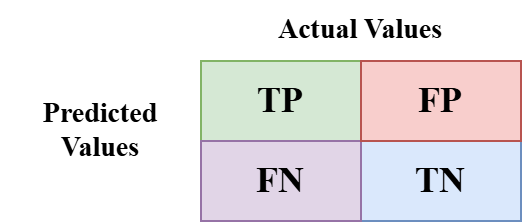
\includegraphics[width=0.6\textwidth,height=0.2\textwidth]{figures/figure6.png}
\caption{Confusion Matrix}\label{Fig6}
\end{figure}

\text{
Acc
}: The proportion of instances correctly classified out of the total.
\begin{equation}\label{eq29}
\text{Acc.} = \frac{\text{TP+TN}}{\text{TP+TN+FP+FN}}
\end{equation}

\text{Pr.}: The ratio of correctly predicted positives to the total predicted positives.
\begin{equation}\label{eq30}
\text{Pr.} = \frac{TP}{TP + FP}
\end{equation}

\text{Rec.}: The ratio of correctly identified positives to the total actual positives.
\begin{equation}\label{eq31}
\text{Rec.} = \frac{TP}{TP + FN}
\end{equation}

\text{F1-Score}: The balanced average of Precision and Recall, measuring a method's overall performance.
\begin{equation}\label{eq32}
\text{F1.} = 2 \times \frac{\text{Pr.} \times \text{Recall}}{\text{Pr.} + \text{Rec.}}
\end{equation}

\text Receiver Operating Characteristic Area Under the Curve: Represents the ability of the method to distinguish between positive and negative classes. 

\text{FPR}: The proportion of normal (negative) instances incorrectly classified as malicious (positive), indicating the false alarm rate.
\begin{equation}\label{eq33}
\text{FPR} = \frac{\text{FP}}{\text{FP} + \text{TN}}
\end{equation}
